In this section, we describe the data-sets we worked with, formally define the user dissatisfaction function, and show how to obtain from it the performance metric used to evaluate the different policies that we will define in the next section.

\subsection{Data-Sets}

Our analysis relies on three different data-sets. First, we have a list of all rentals and returns for which the existing non-dynamic incentive scheme awarded points (as well as whether the point was awarded for the rental, the return, or both), each of which comes with the time at which it occurred \cite{citibikeInternal}. Second, we have a list of all rides in the system with origin location, destination location, and respective times of the start and the end of the trip (\cite{citibikedata}). Finally, we have for each minute and each station in the system, the number of bikes reported to be at the station at that time (\cite{citibikejson}).

EXPLAIN TESTING PERIOD (WHAT TIME DOES DATA COME FROM?)

\subsection{User Dissatisfaction Function}\label{ssec:udf}
The user dissatisfaction functions defined by \cite{raviv2013optimal} map the number of bikes at a station at a given time to the expected number of out-of-stock events over the course of a subsequent time horizon. Formally, the functions assume that two exogeneous stochastic processes\footnote{In our implementation, we assume them to be time-varying Poisson processes.} create arrivals of customers intending to either return or rent bikes at the station. Crucially, these processes are assumed to be independent of the initial condition, that is, of the number of bikes initially at the station. Each intended rental decreases the number of bikes in the station by 1 if a bike is available, i.e., if the number of bikes is at least 1. Intended returns increase the number of bikes by 1 if an empty dock is available at the station, i.e., if the number of bikes is less than the capacity of the station. The number of out-of-stock events then corresponds to the number of the sum of all failed intended returns and rentals, i.e., the expected number of intended returns  when the station is at capacity plus the expected number of intended rentals when the station is empty.

EXPLAIN HOW THE UDF USES DATA TO BE COMPUTED (NO DETAILS).

%In order to 

\begin{figure}
\centering
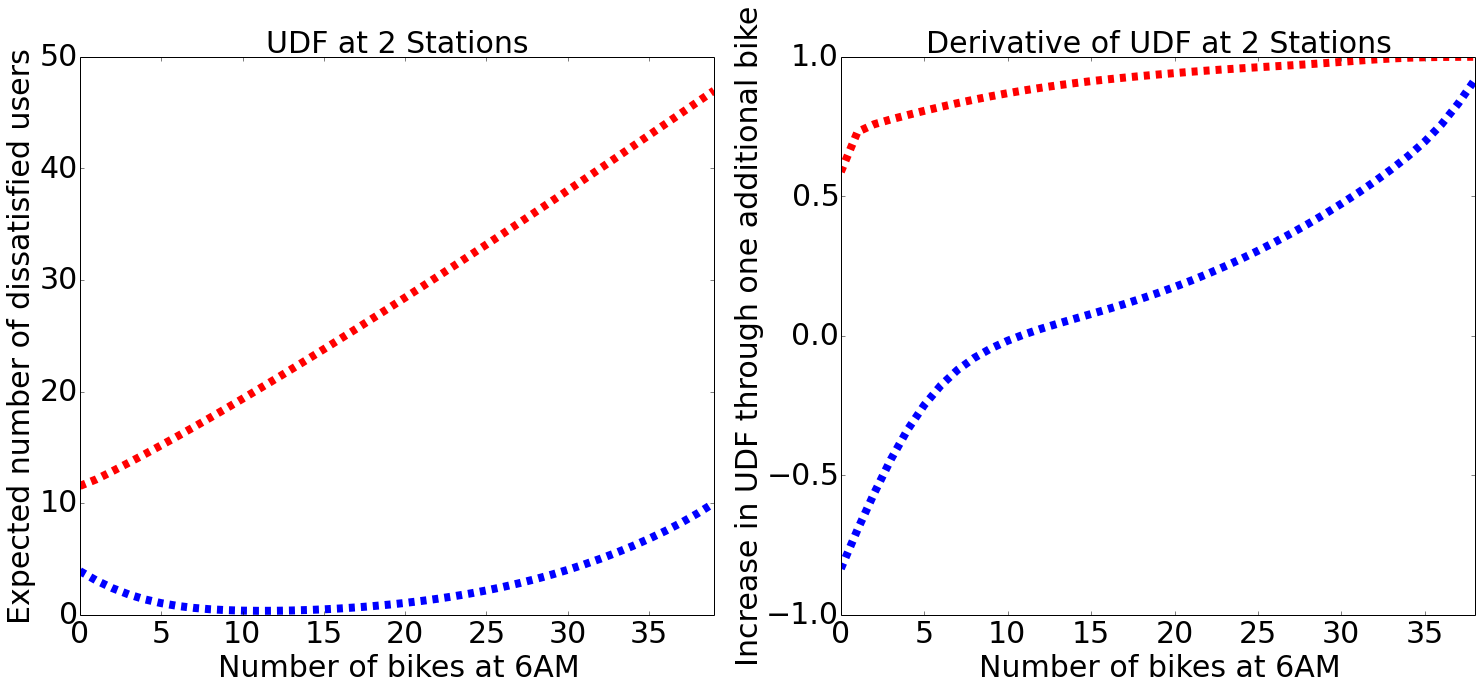
\includegraphics[width=.5\textwidth]{../Plots/UDFandDerivative.png}
\caption{NEEDS A CAPTION}
\label{fig:UDFandDerivative}
\end{figure}

%Formally define the model as defined by \cite{raviv2013optimal}, describe the partition into half-hour intervals, emphasize that there's no point in taking smaller intervals, describe

\subsection{Performance Metrics}

In this section we describe how the user dissatisfaction functions can be used to estimate the efficiency of the Bike Angels incentive scheme. For each incentivized return, we can estimate the reduction in out-of-stock events that the trip caused by computing the discrete derivative of the user dissatisfaction function with respect to one additional bike, evaluated at the number of bikes present in the station before the return. Similarly, for incentivized rentals, the estimated reduction in out-of-stock events equals the difference in the value of the user dissatisfaction function evaluated with one bike less and the actual number of bikes in the station. In Figure \ref{fig:UDFandDerivative}, we display the respective user dissatisfaction functions and the value of the derivatives for two different stations at 6AM. Evaluating the user dissatisfaction functions for every half-hour interval, we estimate the impact of each return/rental on future out-of-stock events by evaluating the derivative of the user dissatisfaction function for that time-interval at the number of bikes present at the time of the return (and similarly for rentals). 

HERE NOTATION WOULD PROBABLY HAVE BEEN GOOD

As we consider the impact of the incentive scheme, it is worthwhile to not only include the impact of each incentivized ride on the user dissatisfaction functions, but also the likelihoods that rides would have occurred without the incentives. EXPLAIN THE FLUID RATES, HOW WE ESTIMATE THEM, CITE o2015data AND EXPLAIN HOW WE DERIVE THE RIDER PROBABILITIES

Finally, we also want to account for the cost of giving incentives. Thus, we associate a fixed cost per awarded incentive point. This corresponds to the operator's cost of monthly rewards in the form of electronic gift cards, membership extensions, etc. \cite{bikeangels}.




%Explain the set up of the problem, data collection methods \\
%Explain the Cost Curve function and what it represents \\
% \\
